% Options for packages loaded elsewhere
\PassOptionsToPackage{unicode}{hyperref}
\PassOptionsToPackage{hyphens}{url}
\PassOptionsToPackage{dvipsnames,svgnames,x11names}{xcolor}
%
\documentclass[
  letterpaper,
  DIV=11,
  numbers=noendperiod]{scrartcl}

\usepackage{amsmath,amssymb}
\usepackage{iftex}
\ifPDFTeX
  \usepackage[T1]{fontenc}
  \usepackage[utf8]{inputenc}
  \usepackage{textcomp} % provide euro and other symbols
\else % if luatex or xetex
  \usepackage{unicode-math}
  \defaultfontfeatures{Scale=MatchLowercase}
  \defaultfontfeatures[\rmfamily]{Ligatures=TeX,Scale=1}
\fi
\usepackage{lmodern}
\ifPDFTeX\else  
    % xetex/luatex font selection
\fi
% Use upquote if available, for straight quotes in verbatim environments
\IfFileExists{upquote.sty}{\usepackage{upquote}}{}
\IfFileExists{microtype.sty}{% use microtype if available
  \usepackage[]{microtype}
  \UseMicrotypeSet[protrusion]{basicmath} % disable protrusion for tt fonts
}{}
\makeatletter
\@ifundefined{KOMAClassName}{% if non-KOMA class
  \IfFileExists{parskip.sty}{%
    \usepackage{parskip}
  }{% else
    \setlength{\parindent}{0pt}
    \setlength{\parskip}{6pt plus 2pt minus 1pt}}
}{% if KOMA class
  \KOMAoptions{parskip=half}}
\makeatother
\usepackage{xcolor}
\setlength{\emergencystretch}{3em} % prevent overfull lines
\setcounter{secnumdepth}{-\maxdimen} % remove section numbering
% Make \paragraph and \subparagraph free-standing
\makeatletter
\ifx\paragraph\undefined\else
  \let\oldparagraph\paragraph
  \renewcommand{\paragraph}{
    \@ifstar
      \xxxParagraphStar
      \xxxParagraphNoStar
  }
  \newcommand{\xxxParagraphStar}[1]{\oldparagraph*{#1}\mbox{}}
  \newcommand{\xxxParagraphNoStar}[1]{\oldparagraph{#1}\mbox{}}
\fi
\ifx\subparagraph\undefined\else
  \let\oldsubparagraph\subparagraph
  \renewcommand{\subparagraph}{
    \@ifstar
      \xxxSubParagraphStar
      \xxxSubParagraphNoStar
  }
  \newcommand{\xxxSubParagraphStar}[1]{\oldsubparagraph*{#1}\mbox{}}
  \newcommand{\xxxSubParagraphNoStar}[1]{\oldsubparagraph{#1}\mbox{}}
\fi
\makeatother

\usepackage{color}
\usepackage{fancyvrb}
\newcommand{\VerbBar}{|}
\newcommand{\VERB}{\Verb[commandchars=\\\{\}]}
\DefineVerbatimEnvironment{Highlighting}{Verbatim}{commandchars=\\\{\}}
% Add ',fontsize=\small' for more characters per line
\usepackage{framed}
\definecolor{shadecolor}{RGB}{241,243,245}
\newenvironment{Shaded}{\begin{snugshade}}{\end{snugshade}}
\newcommand{\AlertTok}[1]{\textcolor[rgb]{0.68,0.00,0.00}{#1}}
\newcommand{\AnnotationTok}[1]{\textcolor[rgb]{0.37,0.37,0.37}{#1}}
\newcommand{\AttributeTok}[1]{\textcolor[rgb]{0.40,0.45,0.13}{#1}}
\newcommand{\BaseNTok}[1]{\textcolor[rgb]{0.68,0.00,0.00}{#1}}
\newcommand{\BuiltInTok}[1]{\textcolor[rgb]{0.00,0.23,0.31}{#1}}
\newcommand{\CharTok}[1]{\textcolor[rgb]{0.13,0.47,0.30}{#1}}
\newcommand{\CommentTok}[1]{\textcolor[rgb]{0.37,0.37,0.37}{#1}}
\newcommand{\CommentVarTok}[1]{\textcolor[rgb]{0.37,0.37,0.37}{\textit{#1}}}
\newcommand{\ConstantTok}[1]{\textcolor[rgb]{0.56,0.35,0.01}{#1}}
\newcommand{\ControlFlowTok}[1]{\textcolor[rgb]{0.00,0.23,0.31}{\textbf{#1}}}
\newcommand{\DataTypeTok}[1]{\textcolor[rgb]{0.68,0.00,0.00}{#1}}
\newcommand{\DecValTok}[1]{\textcolor[rgb]{0.68,0.00,0.00}{#1}}
\newcommand{\DocumentationTok}[1]{\textcolor[rgb]{0.37,0.37,0.37}{\textit{#1}}}
\newcommand{\ErrorTok}[1]{\textcolor[rgb]{0.68,0.00,0.00}{#1}}
\newcommand{\ExtensionTok}[1]{\textcolor[rgb]{0.00,0.23,0.31}{#1}}
\newcommand{\FloatTok}[1]{\textcolor[rgb]{0.68,0.00,0.00}{#1}}
\newcommand{\FunctionTok}[1]{\textcolor[rgb]{0.28,0.35,0.67}{#1}}
\newcommand{\ImportTok}[1]{\textcolor[rgb]{0.00,0.46,0.62}{#1}}
\newcommand{\InformationTok}[1]{\textcolor[rgb]{0.37,0.37,0.37}{#1}}
\newcommand{\KeywordTok}[1]{\textcolor[rgb]{0.00,0.23,0.31}{\textbf{#1}}}
\newcommand{\NormalTok}[1]{\textcolor[rgb]{0.00,0.23,0.31}{#1}}
\newcommand{\OperatorTok}[1]{\textcolor[rgb]{0.37,0.37,0.37}{#1}}
\newcommand{\OtherTok}[1]{\textcolor[rgb]{0.00,0.23,0.31}{#1}}
\newcommand{\PreprocessorTok}[1]{\textcolor[rgb]{0.68,0.00,0.00}{#1}}
\newcommand{\RegionMarkerTok}[1]{\textcolor[rgb]{0.00,0.23,0.31}{#1}}
\newcommand{\SpecialCharTok}[1]{\textcolor[rgb]{0.37,0.37,0.37}{#1}}
\newcommand{\SpecialStringTok}[1]{\textcolor[rgb]{0.13,0.47,0.30}{#1}}
\newcommand{\StringTok}[1]{\textcolor[rgb]{0.13,0.47,0.30}{#1}}
\newcommand{\VariableTok}[1]{\textcolor[rgb]{0.07,0.07,0.07}{#1}}
\newcommand{\VerbatimStringTok}[1]{\textcolor[rgb]{0.13,0.47,0.30}{#1}}
\newcommand{\WarningTok}[1]{\textcolor[rgb]{0.37,0.37,0.37}{\textit{#1}}}

\providecommand{\tightlist}{%
  \setlength{\itemsep}{0pt}\setlength{\parskip}{0pt}}\usepackage{longtable,booktabs,array}
\usepackage{calc} % for calculating minipage widths
% Correct order of tables after \paragraph or \subparagraph
\usepackage{etoolbox}
\makeatletter
\patchcmd\longtable{\par}{\if@noskipsec\mbox{}\fi\par}{}{}
\makeatother
% Allow footnotes in longtable head/foot
\IfFileExists{footnotehyper.sty}{\usepackage{footnotehyper}}{\usepackage{footnote}}
\makesavenoteenv{longtable}
\usepackage{graphicx}
\makeatletter
\def\maxwidth{\ifdim\Gin@nat@width>\linewidth\linewidth\else\Gin@nat@width\fi}
\def\maxheight{\ifdim\Gin@nat@height>\textheight\textheight\else\Gin@nat@height\fi}
\makeatother
% Scale images if necessary, so that they will not overflow the page
% margins by default, and it is still possible to overwrite the defaults
% using explicit options in \includegraphics[width, height, ...]{}
\setkeys{Gin}{width=\maxwidth,height=\maxheight,keepaspectratio}
% Set default figure placement to htbp
\makeatletter
\def\fps@figure{htbp}
\makeatother

\usepackage{booktabs}
\usepackage{caption}
\usepackage{longtable}
\usepackage{colortbl}
\usepackage{array}
\usepackage{anyfontsize}
\usepackage{multirow}
\KOMAoption{captions}{tableheading}
\makeatletter
\@ifpackageloaded{caption}{}{\usepackage{caption}}
\AtBeginDocument{%
\ifdefined\contentsname
  \renewcommand*\contentsname{Table of contents}
\else
  \newcommand\contentsname{Table of contents}
\fi
\ifdefined\listfigurename
  \renewcommand*\listfigurename{List of Figures}
\else
  \newcommand\listfigurename{List of Figures}
\fi
\ifdefined\listtablename
  \renewcommand*\listtablename{List of Tables}
\else
  \newcommand\listtablename{List of Tables}
\fi
\ifdefined\figurename
  \renewcommand*\figurename{Figure}
\else
  \newcommand\figurename{Figure}
\fi
\ifdefined\tablename
  \renewcommand*\tablename{Table}
\else
  \newcommand\tablename{Table}
\fi
}
\@ifpackageloaded{float}{}{\usepackage{float}}
\floatstyle{ruled}
\@ifundefined{c@chapter}{\newfloat{codelisting}{h}{lop}}{\newfloat{codelisting}{h}{lop}[chapter]}
\floatname{codelisting}{Listing}
\newcommand*\listoflistings{\listof{codelisting}{List of Listings}}
\makeatother
\makeatletter
\makeatother
\makeatletter
\@ifpackageloaded{caption}{}{\usepackage{caption}}
\@ifpackageloaded{subcaption}{}{\usepackage{subcaption}}
\makeatother

\ifLuaTeX
  \usepackage{selnolig}  % disable illegal ligatures
\fi
\usepackage{bookmark}

\IfFileExists{xurl.sty}{\usepackage{xurl}}{} % add URL line breaks if available
\urlstyle{same} % disable monospaced font for URLs
\hypersetup{
  pdftitle={Reproducible-R-Project},
  colorlinks=true,
  linkcolor={blue},
  filecolor={Maroon},
  citecolor={Blue},
  urlcolor={Blue},
  pdfcreator={LaTeX via pandoc}}


\title{Reproducible-R-Project}
\author{}
\date{}

\begin{document}
\maketitle


\subsection{Extinct Mammals}\label{extinct-mammals}

\begin{Shaded}
\begin{Highlighting}[]
\FunctionTok{library}\NormalTok{(tidyverse)}
\end{Highlighting}
\end{Shaded}

\begin{verbatim}
-- Attaching core tidyverse packages ------------------------ tidyverse 2.0.0 --
v dplyr     1.1.4     v readr     2.1.5
v forcats   1.0.0     v stringr   1.5.1
v ggplot2   3.5.1     v tibble    3.2.1
v lubridate 1.9.4     v tidyr     1.3.1
v purrr     1.0.4     
-- Conflicts ------------------------------------------ tidyverse_conflicts() --
x dplyr::filter() masks stats::filter()
x dplyr::lag()    masks stats::lag()
i Use the conflicted package (<http://conflicted.r-lib.org/>) to force all conflicts to become errors
\end{verbatim}

\begin{Shaded}
\begin{Highlighting}[]
\FunctionTok{library}\NormalTok{(ggplot2)}
\FunctionTok{library}\NormalTok{(dplyr)}
\NormalTok{data }\OtherTok{\textless{}{-}} \FunctionTok{read.csv}\NormalTok{(}\StringTok{"/Users/robynborgstrom/Desktop/Git/reproducible{-}R{-}project/Extinct mammal dataset.csv"}\NormalTok{, }\AttributeTok{header =} \ConstantTok{TRUE}\NormalTok{, }\AttributeTok{check.names =} \ConstantTok{TRUE}\NormalTok{)}
\FunctionTok{view}\NormalTok{(data)}
\FunctionTok{colnames}\NormalTok{(data)[}\FunctionTok{is.na}\NormalTok{(}\FunctionTok{colnames}\NormalTok{(data))] }\OtherTok{\textless{}{-}} \StringTok{"Picture"}
\FunctionTok{colnames}\NormalTok{(data)}
\end{Highlighting}
\end{Shaded}

\begin{verbatim}
[1] "Common.name"        "Binomial.name"      "Order"             
[4] "Date.of.extinction" "Former.range"       "Picture"           
\end{verbatim}

\begin{Shaded}
\begin{Highlighting}[]
\NormalTok{data}\OtherTok{\textless{}{-}}\FunctionTok{subset}\NormalTok{(data, }\AttributeTok{select =} \SpecialCharTok{{-}}\NormalTok{Picture)}

\FunctionTok{colnames}\NormalTok{(data)}
\end{Highlighting}
\end{Shaded}

\begin{verbatim}
[1] "Common.name"        "Binomial.name"      "Order"             
[4] "Date.of.extinction" "Former.range"      
\end{verbatim}

\begin{Shaded}
\begin{Highlighting}[]
\NormalTok{extinction\_by\_order }\OtherTok{\textless{}{-}}\NormalTok{ data }\SpecialCharTok{\%\textgreater{}\%}
  \FunctionTok{group\_by}\NormalTok{(Order) }\SpecialCharTok{\%\textgreater{}\%}
  \FunctionTok{summarise}\NormalTok{(}\AttributeTok{Count =} \FunctionTok{n}\NormalTok{()) }\SpecialCharTok{\%\textgreater{}\%}
  \FunctionTok{arrange}\NormalTok{(}\FunctionTok{desc}\NormalTok{(Count))}


\FunctionTok{ggplot}\NormalTok{(extinction\_by\_order, }\FunctionTok{aes}\NormalTok{(}\AttributeTok{x =} \FunctionTok{reorder}\NormalTok{(Order, }\SpecialCharTok{{-}}\NormalTok{Count), }\AttributeTok{y =}\NormalTok{ Count, }\AttributeTok{fill =}\NormalTok{ Order)) }\SpecialCharTok{+}
  \FunctionTok{geom\_bar}\NormalTok{(}\AttributeTok{stat =} \StringTok{"identity"}\NormalTok{) }\SpecialCharTok{+}
  \FunctionTok{labs}\NormalTok{(}\AttributeTok{title =} \StringTok{"Extinct Species by Order"}\NormalTok{,}
       \AttributeTok{x =} \StringTok{"Taxonomic Order"}\NormalTok{,}
       \AttributeTok{y =} \StringTok{"Number of Extinct Species"}\NormalTok{) }\SpecialCharTok{+}
  \FunctionTok{theme}\NormalTok{(}\AttributeTok{axis.text.x =} \FunctionTok{element\_text}\NormalTok{(}\AttributeTok{angle =} \DecValTok{45}\NormalTok{, }\AttributeTok{hjust =} \DecValTok{1}\NormalTok{), }
        \AttributeTok{legend.position =} \StringTok{"none"}\NormalTok{)}
\end{Highlighting}
\end{Shaded}

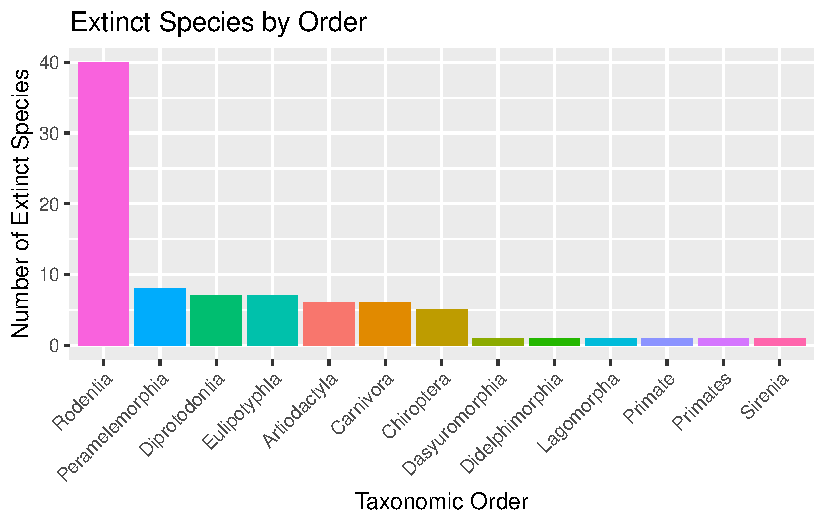
\includegraphics{Extinct-species-by-region-_files/figure-pdf/unnamed-chunk-2-1.pdf}

\begin{Shaded}
\begin{Highlighting}[]
\FunctionTok{ggplot}\NormalTok{(data, }\FunctionTok{aes}\NormalTok{(}\AttributeTok{x =}\NormalTok{ Date.of.extinction, }\AttributeTok{y =}\NormalTok{ Order)) }\SpecialCharTok{+}
  \FunctionTok{geom\_point}\NormalTok{(}\AttributeTok{color =} \StringTok{"blue"}\NormalTok{) }\SpecialCharTok{+}
  \FunctionTok{theme\_minimal}\NormalTok{() }\SpecialCharTok{+}
  \FunctionTok{theme}\NormalTok{(}\AttributeTok{axis.text.x =} \FunctionTok{element\_text}\NormalTok{(}\AttributeTok{angle =} \DecValTok{45}\NormalTok{, }\AttributeTok{hjust =} \DecValTok{1}\NormalTok{)) }\SpecialCharTok{+}
  \FunctionTok{labs}\NormalTok{(}\AttributeTok{title =} \StringTok{"Mammal Extinctions Over Time"}\NormalTok{, }\AttributeTok{x =} \StringTok{"Extinction Date"}\NormalTok{, }\AttributeTok{y =} \StringTok{"Order"}\NormalTok{)}
\end{Highlighting}
\end{Shaded}

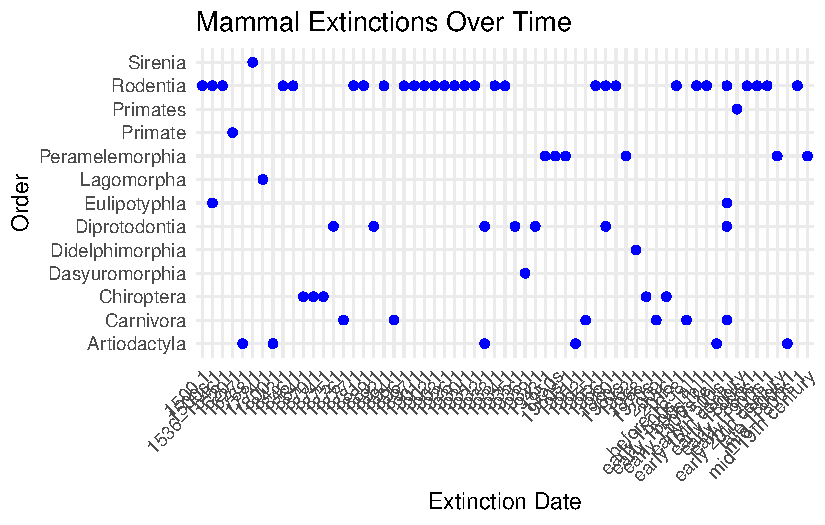
\includegraphics{Extinct-species-by-region-_files/figure-pdf/unnamed-chunk-3-1.pdf}

\begin{Shaded}
\begin{Highlighting}[]
\FunctionTok{library}\NormalTok{(gt)}

\NormalTok{data }\SpecialCharTok{\%\textgreater{}\%}
  \FunctionTok{count}\NormalTok{(Order, }\AttributeTok{sort =} \ConstantTok{TRUE}\NormalTok{) }\SpecialCharTok{\%\textgreater{}\%}
  \FunctionTok{gt}\NormalTok{() }\SpecialCharTok{\%\textgreater{}\%}
  \FunctionTok{tab\_header}\NormalTok{(}\AttributeTok{title =} \StringTok{"Extinct Species by Order"}\NormalTok{)}
\end{Highlighting}
\end{Shaded}

\begin{table}
\caption*{
{\large Extinct Species by Order}
} 
\fontsize{12.0pt}{14.4pt}\selectfont
\begin{tabular*}{\linewidth}{@{\extracolsep{\fill}}lr}
\toprule
Order & n \\ 
\midrule\addlinespace[2.5pt]
Rodentia & 40 \\ 
Peramelemorphia & 8 \\ 
Diprotodontia & 7 \\ 
Eulipotyphla & 7 \\ 
Artiodactyla & 6 \\ 
Carnivora & 6 \\ 
Chiroptera & 5 \\ 
Dasyuromorphia & 1 \\ 
Didelphimorphia & 1 \\ 
Lagomorpha & 1 \\ 
Primate & 1 \\ 
Primates & 1 \\ 
Sirenia & 1 \\ 
\bottomrule
\end{tabular*}
\end{table}

\begin{Shaded}
\begin{Highlighting}[]
\NormalTok{data }\SpecialCharTok{\%\textgreater{}\%}
  \FunctionTok{count}\NormalTok{(Former.range, }\AttributeTok{sort =} \ConstantTok{TRUE}\NormalTok{) }\SpecialCharTok{\%\textgreater{}\%}
  \FunctionTok{gt}\NormalTok{() }\SpecialCharTok{\%\textgreater{}\%}
  \FunctionTok{tab\_header}\NormalTok{(}\AttributeTok{title =} \StringTok{"Extinct Species by Region"}\NormalTok{) }\SpecialCharTok{\%\textgreater{}\%}
  \FunctionTok{cols\_label}\NormalTok{(}\AttributeTok{Former.range =} \StringTok{"Former Range"}\NormalTok{, }\AttributeTok{n =} \StringTok{"Number of Species"}\NormalTok{)}
\end{Highlighting}
\end{Shaded}

\begin{table}
\caption*{
{\large Extinct Species by Region}
} 
\fontsize{12.0pt}{14.4pt}\selectfont
\begin{tabular*}{\linewidth}{@{\extracolsep{\fill}}lr}
\toprule
Former Range & Number of Species \\ 
\midrule\addlinespace[2.5pt]
Australia & 13 \\ 
Hispaniola & 5 \\ 
 & 4 \\ 
Cuba & 4 \\ 
Christmas Island & 3 \\ 
Galápagos Islands & 2 \\ 
Algeria & 1 \\ 
Argentina & 1 \\ 
Argentina, Chile, Brazil, Uruguay, Paraguay & 1 \\ 
Australia (Bramble Cay) & 1 \\ 
Australia (Darling Downs, Queensland) & 1 \\ 
Australia (Flinders and Davenport Ranges) & 1 \\ 
Australia (Great Sandy Desert) & 1 \\ 
Australia (Kangaroo Island and the Younghusband Peninsula) & 1 \\ 
Australia (Nullarbor Plain) & 1 \\ 
Australia (Queensland) & 1 \\ 
Australia (Queensland, New South Wales) & 1 \\ 
Australia (central Western Australia) & 1 \\ 
Australia (eastern coast) & 1 \\ 
Australia (southern half) & 1 \\ 
Australia (west-central) & 1 \\ 
Australia (western and central) & 1 \\ 
Australia, Tasmania & 1 \\ 
Caribbean Sea & 1 \\ 
Central Brazil & 1 \\ 
Commander Islands (Russia, United States) & 1 \\ 
Coronado Islands, Mexico & 1 \\ 
Corsica and Sardinia & 1 \\ 
Cuba (including Isla de la Juventud) & 1 \\ 
Dominican Republic & 1 \\ 
Falkland Islands & 1 \\ 
Fernando de Noronha, Brazil & 1 \\ 
Guam & 1 \\ 
Haiti & 1 \\ 
Hispaniola (currently Dominican Republic) & 1 \\ 
Hispaniola (currently Haiti and the Dominican Republic) & 1 \\ 
Hispaniola; introduced to Puerto Rico, Saint Thomas Island, Saint Croix, U.S. Virgin Islands and Mona Island & 1 \\ 
In green & 1 \\ 
Isla Todos Santos, Mexico & 1 \\ 
Islas Marías, Mexico & 1 \\ 
Jamaica & 1 \\ 
Japan, Korea, Russia & 1 \\ 
Madagascar & 1 \\ 
Martinique & 1 \\ 
Palau & 1 \\ 
Percy Islands (Australia) & 1 \\ 
Peru & 1 \\ 
Puerto Rico, Vieques Island, Saint John, U.S. Virgin Islands, and Saint Thomas, U.S. Virgin Islands & 1 \\ 
Réunion, Mauritius & 1 \\ 
Saint Lucia & 1 \\ 
Saint Vincent & 1 \\ 
San Pedro Nolasco Island, Mexico & 1 \\ 
Santa Cruz Island (Galápagos) & 1 \\ 
Sint Eustatius and Saint Kitts and Nevis & 1 \\ 
Swan Islands, Honduras & 1 \\ 
Thailand & 1 \\ 
United States (Maine, Massachusetts) and Canada (New Brunswick, Newfoundland) & 1 \\ 
Vieques Island, Puerto Rico & 1 \\ 
West Timor, Indonesia & 1 \\ 
Yemen & 1 \\ 
\bottomrule
\end{tabular*}
\end{table}

\begin{Shaded}
\begin{Highlighting}[]
\NormalTok{earliest }\OtherTok{\textless{}{-}}\NormalTok{ data }\SpecialCharTok{\%\textgreater{}\%} \FunctionTok{filter}\NormalTok{(Date.of.extinction }\SpecialCharTok{==} \FunctionTok{min}\NormalTok{(Date.of.extinction, }\AttributeTok{na.rm =} \ConstantTok{TRUE}\NormalTok{))}
\NormalTok{latest }\OtherTok{\textless{}{-}}\NormalTok{ data }\SpecialCharTok{\%\textgreater{}\%} \FunctionTok{filter}\NormalTok{(Date.of.extinction }\SpecialCharTok{==} \FunctionTok{max}\NormalTok{(Date.of.extinction, }\AttributeTok{na.rm =} \ConstantTok{TRUE}\NormalTok{))}

\FunctionTok{rbind}\NormalTok{(earliest, latest) }\SpecialCharTok{\%\textgreater{}\%}
  \FunctionTok{select}\NormalTok{(Common.name, Binomial.name, Date.of.extinction, Former.range) }\SpecialCharTok{\%\textgreater{}\%}
  \FunctionTok{gt}\NormalTok{() }\SpecialCharTok{\%\textgreater{}\%}
  \FunctionTok{tab\_header}\NormalTok{(}\AttributeTok{title =} \StringTok{"Earliest and Latest Extinctions"}\NormalTok{) }\SpecialCharTok{\%\textgreater{}\%}
  \FunctionTok{cols\_label}\NormalTok{(}\AttributeTok{Common.name =} \StringTok{"Common Name"}\NormalTok{, }
             \AttributeTok{Binomial.name =} \StringTok{"Scientific Name"}\NormalTok{, }
             \AttributeTok{Date.of.extinction =} \StringTok{"Year of Extinction"}\NormalTok{, }
             \AttributeTok{Former.range =} \StringTok{"Former Range"}\NormalTok{)}
\end{Highlighting}
\end{Shaded}

\begin{table}
\caption*{
{\large Earliest and Latest Extinctions}
} 
\fontsize{12.0pt}{14.4pt}\selectfont
\begin{tabular*}{\linewidth}{@{\extracolsep{\fill}}llll}
\toprule
Common Name & Scientific Name & Year of Extinction & Former Range \\ 
\midrule\addlinespace[2.5pt]
Vespucci's rodent & Noronhomys vespucciiCarleton and Olson, 1999 & 1500 1 & Fernando de Noronha, Brazil \\ 
New South Wales barred bandicoot[16] & Perameles fasciataGray, 1841 & mid-19th century & Australia \\ 
Southwestern barred bandicoot[16] & Perameles myosurosWagner, 1841 & mid-19th century & Australia \\ 
Southern barred bandicoot[16] & Perameles notinaThomas, 1922 & mid-19th century & Australia \\ 
\bottomrule
\end{tabular*}
\end{table}




\end{document}
